% Options for packages loaded elsewhere
\PassOptionsToPackage{unicode}{hyperref}
\PassOptionsToPackage{hyphens}{url}
%
\documentclass[
  17pt,
  letterpaper,
  ignorenonframetext,
  aspectratio=169,
]{beamer}
\usepackage{pgfpages}
\setbeamertemplate{caption}[numbered]
\setbeamertemplate{caption label separator}{: }
\setbeamercolor{caption name}{fg=normal text.fg}
\beamertemplatenavigationsymbolsempty
% Prevent slide breaks in the middle of a paragraph
\widowpenalties 1 10000
\raggedbottom
\setbeamertemplate{part page}{
  \centering
  \begin{beamercolorbox}[sep=16pt,center]{part title}
    \usebeamerfont{part title}\insertpart\par
  \end{beamercolorbox}
}
\setbeamertemplate{section page}{
  \centering
  \begin{beamercolorbox}[sep=12pt,center]{part title}
    \usebeamerfont{section title}\insertsection\par
  \end{beamercolorbox}
}
\setbeamertemplate{subsection page}{
  \centering
  \begin{beamercolorbox}[sep=8pt,center]{part title}
    \usebeamerfont{subsection title}\insertsubsection\par
  \end{beamercolorbox}
}
\AtBeginPart{
  \frame{\partpage}
}
\AtBeginSection{
  \ifbibliography
  \else
    \frame{\sectionpage}
  \fi
}
\AtBeginSubsection{
  \frame{\subsectionpage}
}

\usepackage{amsmath,amssymb}
\usepackage{lmodern}
\usepackage{iftex}
\ifPDFTeX
  \usepackage[T1]{fontenc}
  \usepackage[utf8]{inputenc}
  \usepackage{textcomp} % provide euro and other symbols
\else % if luatex or xetex
  \usepackage{unicode-math}
  \defaultfontfeatures{Scale=MatchLowercase}
  \defaultfontfeatures[\rmfamily]{Ligatures=TeX,Scale=1}
  \setmainfont[BoldFont = SF Pro Text Semibold, Scale =
MatchLowercase]{SF Pro Text Light}
\fi
\usecolortheme{wolverine}
\usefonttheme{serif} % use mainfont rather than sansfont for slide text
\useinnertheme{default}
\useoutertheme{miniframes}
% Use upquote if available, for straight quotes in verbatim environments
\IfFileExists{upquote.sty}{\usepackage{upquote}}{}
\IfFileExists{microtype.sty}{% use microtype if available
  \usepackage[]{microtype}
  \UseMicrotypeSet[protrusion]{basicmath} % disable protrusion for tt fonts
}{}
\makeatletter
\@ifundefined{KOMAClassName}{% if non-KOMA class
  \IfFileExists{parskip.sty}{%
    \usepackage{parskip}
  }{% else
    \setlength{\parindent}{0pt}
    \setlength{\parskip}{6pt plus 2pt minus 1pt}}
}{% if KOMA class
  \KOMAoptions{parskip=half}}
\makeatother
\usepackage{xcolor}
\newif\ifbibliography
\setlength{\emergencystretch}{3em} % prevent overfull lines
\setcounter{secnumdepth}{-\maxdimen} % remove section numbering


\providecommand{\tightlist}{%
  \setlength{\itemsep}{0pt}\setlength{\parskip}{0pt}}\usepackage{longtable,booktabs,array}
\usepackage{calc} % for calculating minipage widths
\usepackage{caption}
% Make caption package work with longtable
\makeatletter
\def\fnum@table{\tablename~\thetable}
\makeatother
\usepackage{graphicx}
\makeatletter
\def\maxwidth{\ifdim\Gin@nat@width>\linewidth\linewidth\else\Gin@nat@width\fi}
\def\maxheight{\ifdim\Gin@nat@height>\textheight\textheight\else\Gin@nat@height\fi}
\makeatother
% Scale images if necessary, so that they will not overflow the page
% margins by default, and it is still possible to overwrite the defaults
% using explicit options in \includegraphics[width, height, ...]{}
\setkeys{Gin}{width=\maxwidth,height=\maxheight,keepaspectratio}
% Set default figure placement to htbp
\makeatletter
\def\fps@figure{htbp}
\makeatother

\captionsetup[figure]{labelformat=empty}
\usepackage{pgfpages}
\setbeamertemplate{itemize item}[circle]
\setbeamertemplate{footline}[frame number]{}
\mode<handout>{\pgfpagesuselayout{6 on 1}[letterpaper, border shrink=8mm]}
\AtBeginSection{%
   \begin{frame}
       \tableofcontents[currentsection]
   \end{frame}
}
\makeatletter
\makeatother
\makeatletter
\makeatother
\makeatletter
\@ifpackageloaded{caption}{}{\usepackage{caption}}
\AtBeginDocument{%
\ifdefined\contentsname
  \renewcommand*\contentsname{Table of contents}
\else
  \newcommand\contentsname{Table of contents}
\fi
\ifdefined\listfigurename
  \renewcommand*\listfigurename{List of Figures}
\else
  \newcommand\listfigurename{List of Figures}
\fi
\ifdefined\listtablename
  \renewcommand*\listtablename{List of Tables}
\else
  \newcommand\listtablename{List of Tables}
\fi
\ifdefined\figurename
  \renewcommand*\figurename{Figure}
\else
  \newcommand\figurename{Figure}
\fi
\ifdefined\tablename
  \renewcommand*\tablename{Table}
\else
  \newcommand\tablename{Table}
\fi
}
\@ifpackageloaded{float}{}{\usepackage{float}}
\floatstyle{ruled}
\@ifundefined{c@chapter}{\newfloat{codelisting}{h}{lop}}{\newfloat{codelisting}{h}{lop}[chapter]}
\floatname{codelisting}{Listing}
\newcommand*\listoflistings{\listof{codelisting}{List of Listings}}
\makeatother
\makeatletter
\@ifpackageloaded{caption}{}{\usepackage{caption}}
\@ifpackageloaded{subcaption}{}{\usepackage{subcaption}}
\makeatother
\makeatletter
\@ifpackageloaded{tcolorbox}{}{\usepackage[many]{tcolorbox}}
\makeatother
\makeatletter
\@ifundefined{shadecolor}{\definecolor{shadecolor}{rgb}{.97, .97, .97}}
\makeatother
\makeatletter
\makeatother
\ifLuaTeX
  \usepackage{selnolig}  % disable illegal ligatures
\fi
\IfFileExists{bookmark.sty}{\usepackage{bookmark}}{\usepackage{hyperref}}
\IfFileExists{xurl.sty}{\usepackage{xurl}}{} % add URL line breaks if available
\urlstyle{same} % disable monospaced font for URLs
\hypersetup{
  pdftitle={Knowledge and Reality, Lecture 04},
  pdfauthor={Brian Weatherson},
  hidelinks,
  pdfcreator={LaTeX via pandoc}}

\title{Knowledge and Reality, Lecture 04}
\author{Brian Weatherson}
\date{2022-09-12}

\begin{document}
\frame{\titlepage}
\ifdefined\Shaded\renewenvironment{Shaded}{\begin{tcolorbox}[borderline west={3pt}{0pt}{shadecolor}, interior hidden, breakable, sharp corners, enhanced, frame hidden, boxrule=0pt]}{\end{tcolorbox}}\fi

\hypertarget{review}{%
\section{Review}\label{review}}

\begin{frame}{Is Testimony a Basic Knowledge Source}
\protect\hypertarget{is-testimony-a-basic-knowledge-source}{}
Lots of reasons to think it might not be.

\begin{enumerate}[<+->]
\tightlist
\item
  People deceive us, either intentionally or unintentionally.
\item
  Sources differ.
\item
  Testimony isn't independent of other sources.
\end{enumerate}
\end{frame}

\begin{frame}{Is Testimony a Basic Knowledge Source}
\protect\hypertarget{is-testimony-a-basic-knowledge-source-1}{}
None of these are conclusive, since they all overgenerate.

\begin{enumerate}[<+->]
\tightlist
\item
  Looks can be deceiving.
\item
  Things look different from different angles.
\item
  Inference isn't independent.
\end{enumerate}
\end{frame}

\begin{frame}{Why Might Testimony be Basic}
\protect\hypertarget{why-might-testimony-be-basic}{}
\begin{enumerate}[<+->]
\tightlist
\item
  In practice we act like it is.
\item
  It would be impossible to not act like it is (perhaps especially in
  childhood).
\item
  Language must be mostly correct in order to work.
\end{enumerate}
\end{frame}

\begin{frame}{Plan for Today}
\protect\hypertarget{plan-for-today}{}
\begin{enumerate}[<+->]
\tightlist
\item
  Happy to answer any questions about the reading.
\item
  But my priority is explaining background, because this intersects a
  lot of debates inside and outside philosophy.
\end{enumerate}
\end{frame}

\hypertarget{reductionism}{%
\section{Reductionism}\label{reductionism}}

\begin{frame}{Two Approaches to Testimony}
\protect\hypertarget{two-approaches-to-testimony}{}
\begin{enumerate}[<+->]
\tightlist
\item
  Reductionism
\item
  Anti-Reductionism
\end{enumerate}
\end{frame}

\begin{frame}{Anti-Reductionism}
\protect\hypertarget{anti-reductionism}{}
This is basically the testimony is a pramana position.
\end{frame}

\begin{frame}{Anti-Reductionism}
\protect\hypertarget{anti-reductionism-1}{}
Two aspects, that don't need to go together.

\begin{itemize}[<+->]
\tightlist
\item
  Evaluative: People can do well by taking speakers at their word.
\item
  Psychological: People in fact take speakers at their word.
\end{itemize}
\end{frame}

\begin{frame}{Motivations for Anti-Reductionism}
\protect\hypertarget{motivations-for-anti-reductionism}{}
\begin{itemize}[<+->]
\tightlist
\item
  Mostly carried over (well, belatedly rediscovered) from Indian
  traditions.
\item
  But one new motivation, a focus on infants and toddlers.
\item
  They couldn't learn if reductionism were true.
\end{itemize}
\end{frame}

\begin{frame}{Reductionism}
\protect\hypertarget{reductionism-1}{}
Testimony is not a pramana.

\begin{itemize}[<+->]
\tightlist
\item
  It reduces fundamentally to perception + inference.
\end{itemize}
\end{frame}

\begin{frame}{Standard form of testimonial inference}
\protect\hypertarget{standard-form-of-testimonial-inference}{}
\begin{enumerate}[<+->]
\tightlist
\item
  Speaker said that p.
\item
  This speaker is generally reliable (perhaps known, perhaps reasoned
  from background).
\item
  This speaker has no reason to deceive.
\item
  So, probably, p.
\end{enumerate}
\end{frame}

\begin{frame}{Two Distinct Claims}
\protect\hypertarget{two-distinct-claims}{}
\begin{itemize}[<+->]
\tightlist
\item
  Good hearers go through something like this inference.
\item
  Real hearers (typically) go through something like this inference.
\end{itemize}
\end{frame}

\begin{frame}{Sperber et al}
\protect\hypertarget{sperber-et-al}{}
Both those claims are true.
\end{frame}

\hypertarget{rationality-wars}{%
\section{Rationality Wars}\label{rationality-wars}}

\begin{frame}{A Very Brief History}
\protect\hypertarget{a-very-brief-history}{}
\begin{itemize}[<+->]
\tightlist
\item
  Late C20 psychology included included big trend of arguing that people
  are much less rational than they seem.
\item
  Early C21 has featured some pushback to this.
\item
  This paper is (a kind of important) part of the pushback.
\end{itemize}
\end{frame}

\begin{frame}{Heuristics and Biases}
\protect\hypertarget{heuristics-and-biases}{}
\begin{figure}

{\centering 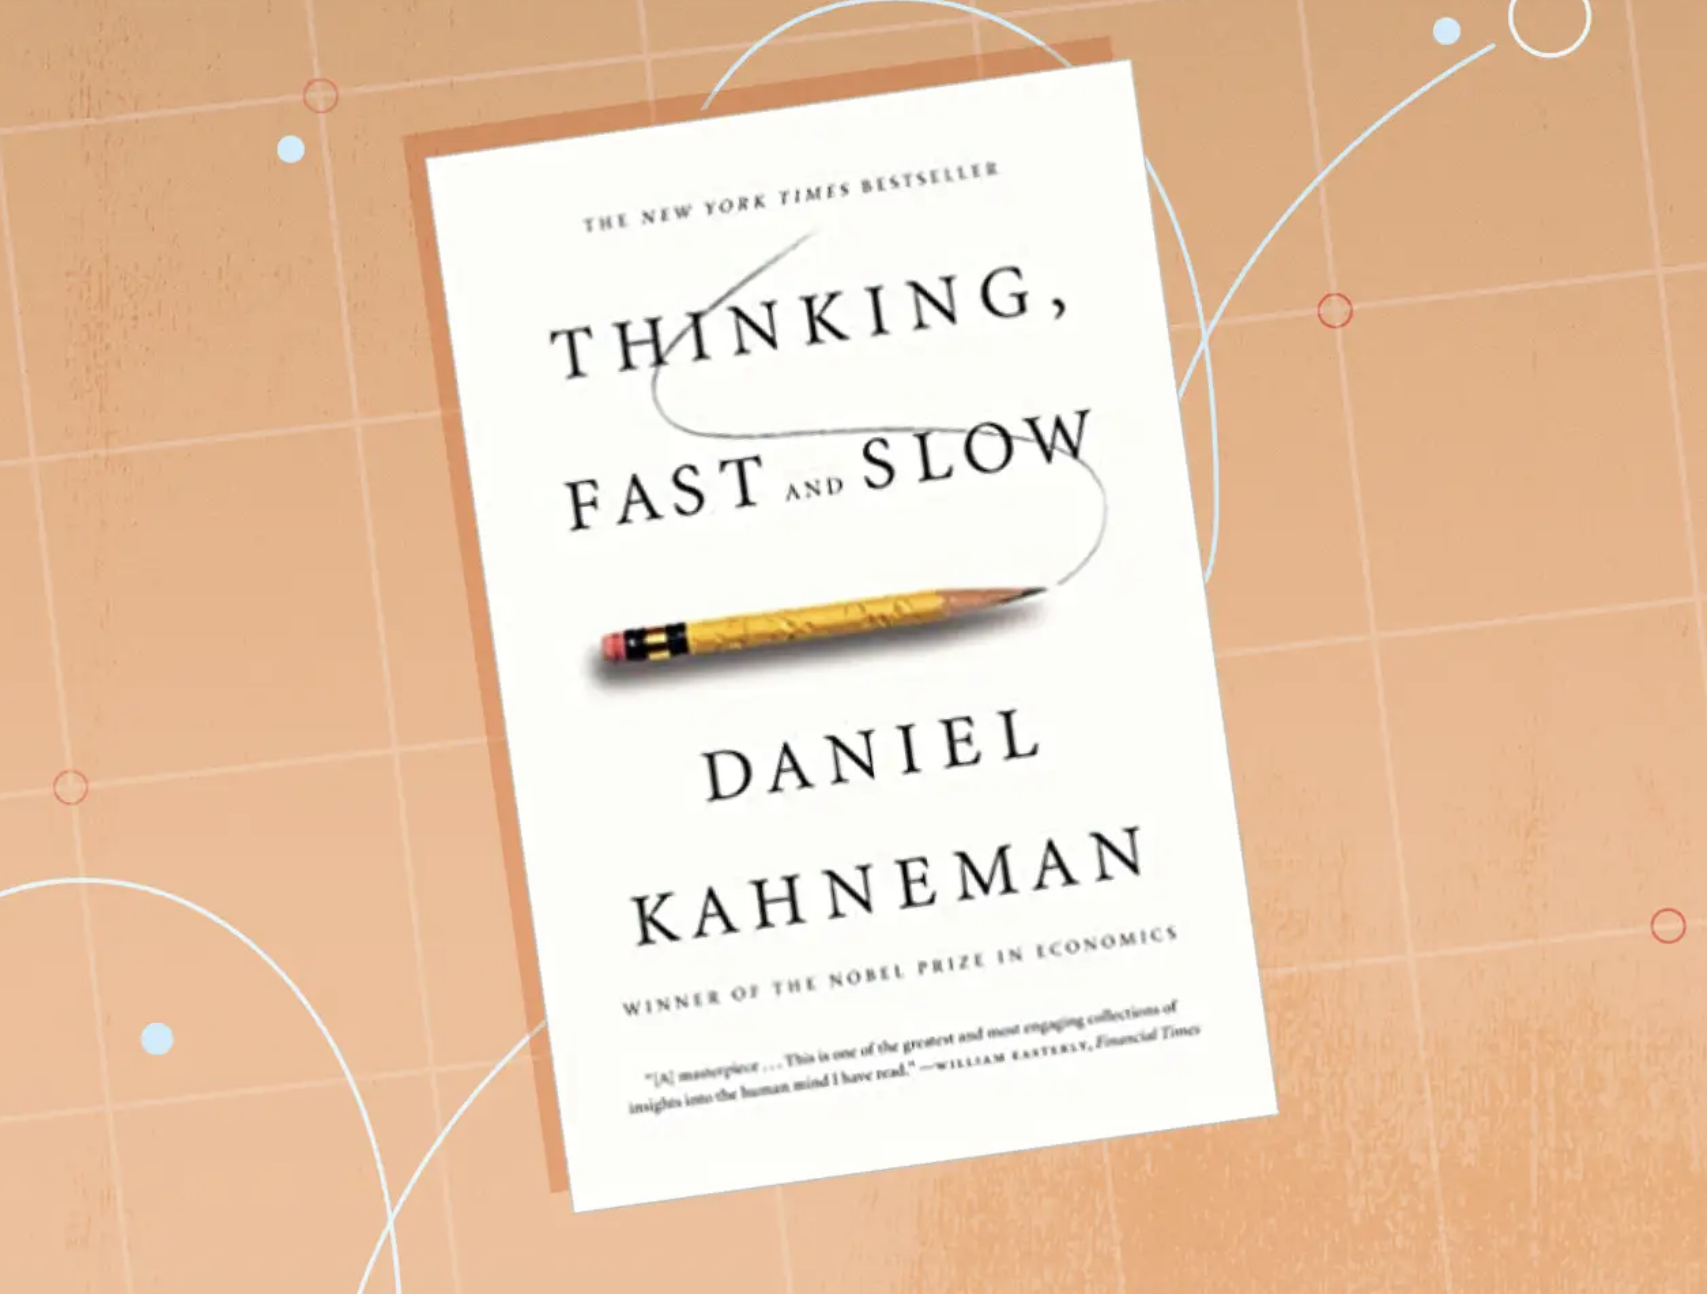
\includegraphics[width=\textwidth,height=0.6\textheight]{../images/kahneman.png}

}

\caption{Thinking Fast and Slow, by Daniel Kahneman}

\end{figure}
\end{frame}

\begin{frame}{Heuristics and Biases}
\protect\hypertarget{heuristics-and-biases-1}{}
\begin{itemize}[<+->]
\tightlist
\item
  Work Kahneman did with Amos Tversky.
\item
  What looks like intelligent behavior is mostly a set of heuristics,
  i.e., short-cuts.
\end{itemize}
\end{frame}

\begin{frame}{System 1 and System 2}
\protect\hypertarget{system-1-and-system-2}{}
\begin{itemize}[<+->]
\tightlist
\item
  Kahneman's own view is that there is a core of something like
  traditional rationality.
\item
  This is system 2, the slow of ``Thinking Fast and Slow''.
\item
  But most of what we do, and everything we do fast, is basically
  automatic.
\end{itemize}
\end{frame}

\begin{frame}{More Radical Views}
\protect\hypertarget{more-radical-views}{}
\begin{itemize}[<+->]
\tightlist
\item
  Drop, or minimise, the existence of system 2.
\item
  It's all just automatic heuristics that have evolved to be useful.
\end{itemize}
\end{frame}

\begin{frame}{Dan Gilbert}
\protect\hypertarget{dan-gilbert}{}
\begin{figure}

{\centering 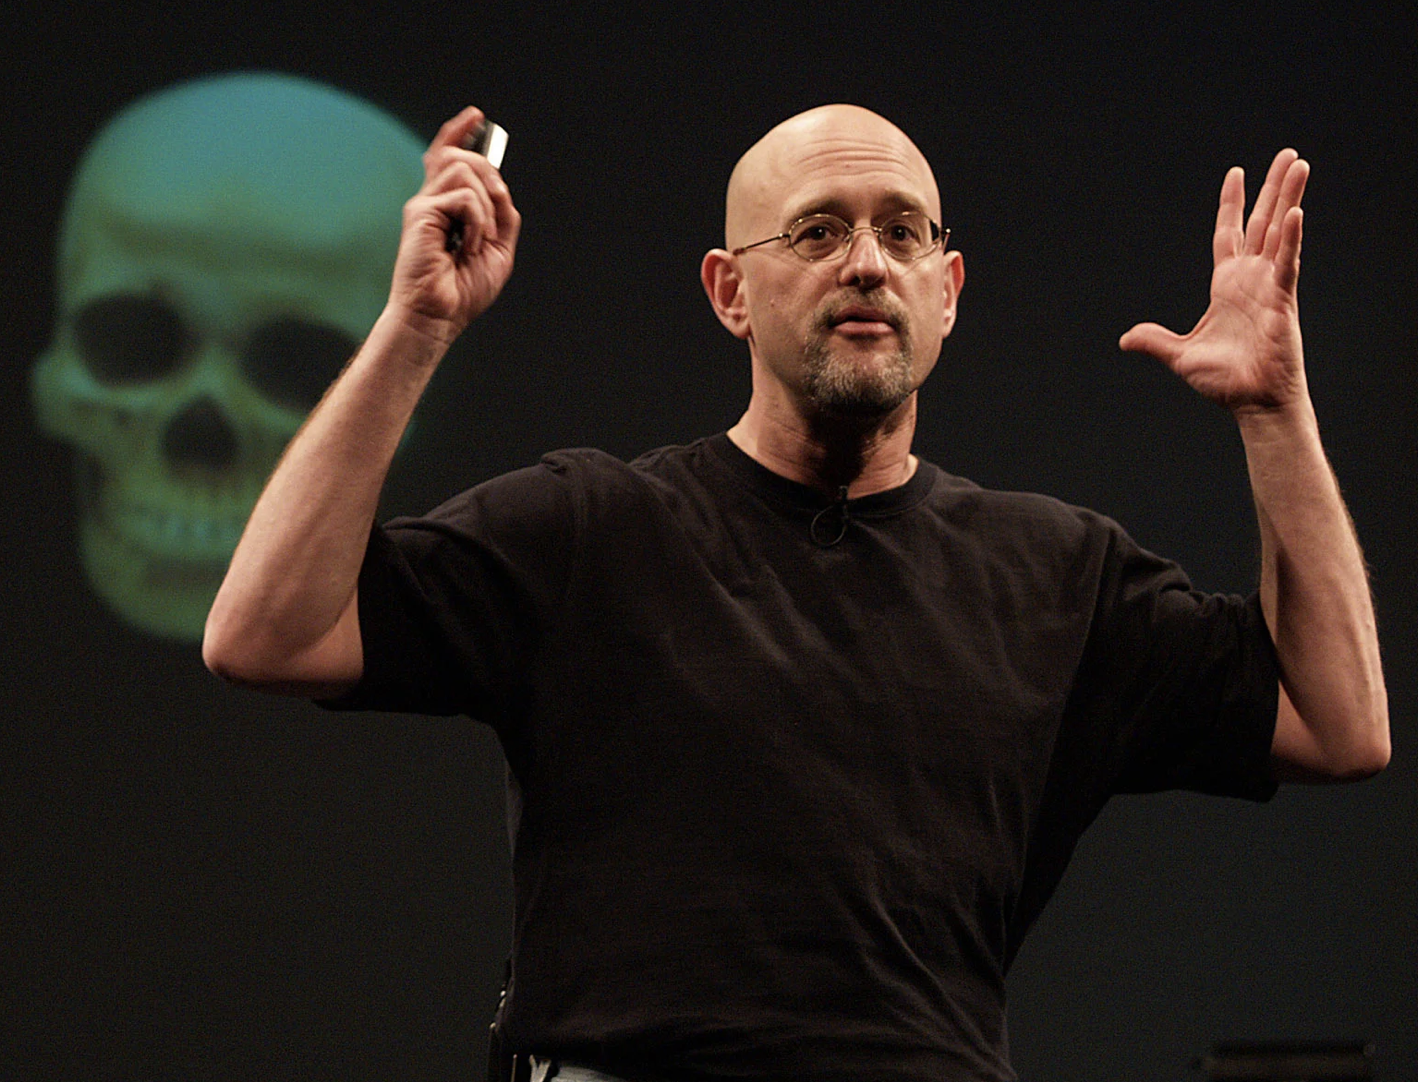
\includegraphics[width=\textwidth,height=0.6\textheight]{../images/gilbert.png}

}

\caption{Daniel Gilbert}

\end{figure}
\end{frame}

\begin{frame}{A Famous Experiment}
\protect\hypertarget{a-famous-experiment}{}
Show people a bunch of sentences for short amount of time each.

\begin{itemize}[<+->]
\tightlist
\item
  Tell them the ones in black will be true, and the ones in red false.
\item
  Make the content of each (black and red) plausible, but not something
  they know about.
\end{itemize}
\end{frame}

\begin{frame}{Later that day\ldots{}}
\protect\hypertarget{later-that-day}{}
Show them the sentences again, and ask whether they are true or false.

\begin{itemize}[<+->]
\tightlist
\item
  They tend to say yes to both the ones in black and the ones in red.
\end{itemize}
\end{frame}

\begin{frame}{What is Going On?}
\protect\hypertarget{what-is-going-on}{}
Why do \textbf{you} think that we might see these results.
\end{frame}

\begin{frame}{What is Going On?}
\protect\hypertarget{what-is-going-on-1}{}
Gilbert's hypothesis (which he attributes to Spinoza):

\begin{itemize}[<+->]
\tightlist
\item
  Understanding language involves first taking something to be true,
  then (perhaps) questioning whether it is.
\item
  This is a really strong form of (psychological) anti-reductionism.
\end{itemize}
\end{frame}

\begin{frame}{Pushback}
\protect\hypertarget{pushback}{}
\begin{itemize}[<+->]
\tightlist
\item
  We'll get to this in more detail, but the very short version is that
  the `automatic' behavior might be sensible allocation of scarce
  cognitive resources. More on this to follow.
\end{itemize}
\end{frame}

\hypertarget{cultural-evolution}{%
\section{Cultural Evolution}\label{cultural-evolution}}

\begin{frame}{Two Theories of Cultural Evolution}
\protect\hypertarget{two-theories-of-cultural-evolution}{}
\begin{enumerate}[<+->]
\tightlist
\item
  Copying
\item
  Rational adoption
\end{enumerate}
\end{frame}

\begin{frame}{Two Theories of Cultural Evolution}
\protect\hypertarget{two-theories-of-cultural-evolution-1}{}
\begin{itemize}[<+->]
\tightlist
\item
  These aren't exhaustive, plenty of other stories too.
\item
  The Australian philosopher of biology Kim Sterelny calls the schools
  that center these ideas the ``California school'' and the ``Paris
  School''.
\item
  This paper is an important text in the Paris school approach.
\end{itemize}
\end{frame}

\begin{frame}{Paris School}
\protect\hypertarget{paris-school}{}
\begin{itemize}[<+->]
\tightlist
\item
  The key moves in cultural evolution are rational.
\item
  But they aren't always conscious.
\end{itemize}
\end{frame}

\begin{frame}{Why Replication}
\protect\hypertarget{why-replication}{}
\begin{itemize}[<+->]
\tightlist
\item
  We see someone doing X and succeeding in a certain way.
\item
  We want to succeed in that same way.
\item
  We infer, fallibly, sub-consciously, that the are succeeding because
  of X.
\item
  So we do X as well.
\end{itemize}
\end{frame}

\begin{frame}{Distinctive Features of Paris}
\protect\hypertarget{distinctive-features-of-paris}{}
\begin{itemize}[<+->]
\tightlist
\item
  We won't always make that inference.
\item
  We will tinker if we have reason to believe that we can improve.
\item
  We will reject if we have reason to believe that X won't work for us.
\end{itemize}
\end{frame}

\begin{frame}{To be Sure}
\protect\hypertarget{to-be-sure}{}
\begin{itemize}[<+->]
\tightlist
\item
  The believers in replication know that people are not robots, and
  think for themselves.
\item
  The believers in rational adoption know that we make mistakes.
\item
  But there is a difference in emphasis, that is interesting.
\end{itemize}
\end{frame}

\begin{frame}{Application to Misinformation}
\protect\hypertarget{application-to-misinformation}{}
\begin{itemize}[<+->]
\tightlist
\item
  The replication approach makes misinformation seem like a big
  political problem.
\item
  And the evidence that people are bad at correcting misinformation
  might push you towards the replication approach.
\end{itemize}
\end{frame}

\begin{frame}{Two Parisian Responses}
\protect\hypertarget{two-parisian-responses}{}
\begin{enumerate}[<+->]
\tightlist
\item
  People don't actually believe that much misinformation, but pretend to
  do so as a social/political signal. E.g., almost no one really
  believed `Pizzagate'.
\item
  Misinformation is a demand side problem; people (rationally!) want
  rationalisations for things they want to be true.
\end{enumerate}
\end{frame}

\begin{frame}{Citations}
\protect\hypertarget{citations}{}
The following bits of text link to the relevant papers.

\begin{itemize}[<+->]
\tightlist
\item
  \href{https://www.sciencedirect.com/science/article/pii/S1369848616301078\#fn14}{Sterelny
  on the two schools}
\item
  \href{https://www.cambridge.org/core/journals/american-political-science-review/article/analytical-democratic-theory-a-microfoundational-approach/739A9A928A99A47994E4585059B03398}{Mercier
  and colleagues on misinformation}
\item
  \href{https://www.cambridge.org/core/journals/economics-and-philosophy/article/marketplace-of-rationalizations/41FB096344BD344908C7C992D0C0C0DC}{Williams
  on the marketplace of rationalisations}
\end{itemize}
\end{frame}

\hypertarget{back-to-testimony-and-fraud}{%
\section{Back to Testimony, and
Fraud}\label{back-to-testimony-and-fraud}}

\begin{frame}{Credit Card Fraud}
\protect\hypertarget{credit-card-fraud}{}
Credit card fraud is a multi-billion dollar problem, and the costs are
largely borne by card issuers.

\begin{itemize}[<+->]
\tightlist
\item
  If you were a credit card issuer, what would you do about this?
\end{itemize}
\end{frame}

\begin{frame}{Short Term Effects}
\protect\hypertarget{short-term-effects}{}
\begin{itemize}[<+->]
\tightlist
\item
  Each genuine transaction makes you some money.
\item
  Each fraudulent transaction costs you much more money.
\end{itemize}
\end{frame}

\begin{frame}{Long Term Effects}
\protect\hypertarget{long-term-effects}{}
\begin{itemize}[<+->]
\tightlist
\item
  If fraud detection is too onerous, people will stop using your card.
\item
  If there is a kind of fraud you never catch, people will keep carrying
  out that fraud.
\end{itemize}
\end{frame}

\begin{frame}{Four Kinds of Checks}
\protect\hypertarget{four-kinds-of-checks}{}
\begin{itemize}[<+->]
\tightlist
\item
  User based
\item
  Purchase based
\item
  Interaction of the two
\item
  Random
\end{itemize}
\end{frame}

\begin{frame}{Optimal Amount of Fraud}
\protect\hypertarget{optimal-amount-of-fraud}{}
Should you be aiming for zero fraud?

\begin{itemize}[<+->]
\tightlist
\item
  No!
\end{itemize}
\end{frame}

\begin{frame}{Basic Idea of Fraud Detection System}
\protect\hypertarget{basic-idea-of-fraud-detection-system}{}
\begin{itemize}[<+->]
\tightlist
\item
  Really rough and ready check on each transaction.
\item
  More careful check on things that get red flagged.
\item
  But for trusted customers, even a few red flags can be ignored.
\end{itemize}
\end{frame}

\begin{frame}{Vigilance}
\protect\hypertarget{vigilance}{}
Humans should be, and to some extent are, just like that.

\begin{itemize}[<+->]
\tightlist
\item
  Everything we hear gets a really rough check over.
\item
  Red flagged assertions get checked more closely.
\end{itemize}
\end{frame}

\begin{frame}{Vigilance}
\protect\hypertarget{vigilance-1}{}
My favorite example: walking down a busy street or corridor.

\begin{itemize}[<+->]
\tightlist
\item
  We somehow track everyone, while attending to almost no one.
\item
  Really big question: How on earth do we do this, and can we invent a
  machine that does something similar?
\end{itemize}
\end{frame}

\begin{frame}{Vigilant Hearers}
\protect\hypertarget{vigilant-hearers}{}
Sperber et al think that we are also vigilant in hearing.

\begin{itemize}[<+->]
\tightlist
\item
  Everything gets a rough check, almost always subconsciously.
\item
  Some things get more thorough check.
\end{itemize}
\end{frame}

\begin{frame}{Red Flags}
\protect\hypertarget{red-flags}{}
\begin{itemize}[<+->]
\tightlist
\item
  New informants
\item
  Surprising that info is either true or known
\item
  Reason to deceive
\item
  High stakes
\end{itemize}
\end{frame}

\begin{frame}{Big Question}
\protect\hypertarget{big-question}{}
Is this plausible as a model of how human hearers operate?
\end{frame}

\begin{frame}{For Next Time}
\protect\hypertarget{for-next-time}{}
\begin{itemize}[<+->]
\tightlist
\item
  The debate between ``internalism'' and ``externalism'' in
  epistemology.
\end{itemize}
\end{frame}



\end{document}
